\section{Discussion of our results}
\label{sec:discussion}
As we have seen in section~\ref{sec:results}, we have not obtained the 
expected results from our simulations in all cases. In this section we discuss 
some possible changes that we believe will fix these discrepancies.

The section is divided into three parts: A discussion of the effects of making 
the interaction forces velocity dependent, a discussion of parameter values, and a 
discussion of possible errors related to our implementation of the simulation.

\subsection{Adding additional forces}
An obvious possibility when discussing why we do not see the expected results, 
is analysing the forces that comprise the model. Two things become apparent: 
the forces in the model are simplistic, as they are only changing with the relative 
positions (away from the point of repulsion), and none of them are dependent 
on the current velocity of the pedestrians. This gives rise to two types of 
behaviour: pedestrians walking directly towards each other do not try to avoid 
colliding, and pedestrians running towards a wall decelerate at the same rate 
as pedestrians walking towards it. This is illustrated in 
figure~\ref{fig:extra-forces-behaviour}.

\begin{figure}[h]
    \centering
    \subfloat[Pedestrians walking towards each other.]{
        \begin{tikzpicture}[scale=2,>=latex]
             \node (p1) at (-0.5,0.5) [circle,draw] {};
             \node (p2) at ( 0.5,0.5) [circle,draw] {};
             \node (p3) at (-0.5,0) [circle,draw] {};
             \node (p4) at ( 0.5,0) [circle,draw] {};

             \draw[->] (p1) -- +(0.5,0);
             \draw[->] (p2) -- +(-0.5,0);
             \draw[->] (p3) -- (0,0.1);
             \draw[->] (p4) -- (0,-0.1);

            \useasboundingbox (-2,-1) rectangle (2,1);
        \end{tikzpicture}
        \label{subfig:colliding}
        }
    \subfloat[Pedestrians running and walking towards a wall.]{
        \begin{tikzpicture}[scale=2,>=latex]
            \draw[o-o] (-1,1) -- (1,1);
            \node (p1) at (-0.5,0) [circle,draw] {};
            \node (p2) at ( 0.5,0) [circle,draw] {};

            \draw[blue,->] (p1) -- +(0,0.5);
            \draw[blue,->] (p2) -- +(0,0.75);
            \draw[red,->] (p1) -- +(0,-0.25);
            \draw[red,->] (p2) -- +(0,-0.25);
            \useasboundingbox (-2,-1) rectangle (2,1);
        \end{tikzpicture}
        \label{subfig:equal-repulsion}}
    \caption[Behaviour from simplistic forces]{Behaviour from simplistic 
    forces. \subref{subfig:colliding} Pedestrians walking towards each other 
    do not divert to the side (top pair), even though doing to would avoid a 
    collision (bottom pair). \subref{subfig:equal-repulsion} Pedestrians 
    heading towards the wall at different speeds (blue arrows) are repulsed 
    equally (red arrows).}
    \label{fig:extra-forces-behaviour}
\end{figure}

When pedestrians decelerate at the same rate no matter their velocity, they 
will in certain extreme cases (i.e. when they are moving very fast) not 
decelerate enough, and so will move through walls or even each other. Since 
the repulsive forces are exponential in nature, lowering the time step size 
enough for the increasing forces to take effect as the distance becomes 
shorter somewhat mitigates the tendency to walk through walls; however, it is 
not always enough. Adding a velocity-dependent term to the repulsive forces 
could be a remedy for this behaviour. Indeed, adding such a force has been 
seen to improve model predictions when compared to data from real life 
situations \cite{ABconstant}.

Making pedestrians avoid each other might be done by adding a component of the 
repulsive force that is tangential to the direction of the vector between the 
repulsion points. Such a force would be a way to avoid having pedestrians that 
head straight for a collision (as we have seen examples of in our simulations) 
and instead make them sidestep each other, as illustrated in 
figure~\ref{subfig:colliding}. We believe this would improve the results from 
the simulations of corridors that have pedestrians walking in both directions. 
It could also enable pedestrians to navigate around static obstacles, such as 
pillars. While we have not done any simulations involving such obstacles, this 
has been seen in e.g. \cite{tang}. Finally, a tangential force might allow 
pedestrians to navigate along a wall if its target is on the other side of it; 
this could be used to simulate pedestrians trapped in a smoke-filled room 
where the exits are not visible.

Another improvement of adding tangential forces comes from the similarities 
between such forces and frictional forces seen in real life. This would make 
it harder for pedestrians to move through a densely packed crowd, and we 
believe adding such forces would enable us to see the faster-is-slower effect 
in our simulation. This is corroborated by the fact that other articles that 
include this effect incorporate just such a tangential force \cite{self-org}. 
Other effects related to clogging of passages, such as the freezing by heating 
effect might also be more apparent given tangential forces.


\subsection{Parameter values}
The magnitude of the forces in the model depend heavily on the values of the 
various constants that are set as model parameters. This means that choosing 
good model parameters is important to get good results. The parameters we have 
used are obtained from several different articles, and so we cannot be sure 
that our starting point has been a good one. Especially since the parameters 
vary wildly between articles, when they are at all comparable. We have 
attempted to adjust some of the parameters when we have seen strange 
behaviour, such as pedestrians walking through walls, etc. The fact remains, 
though, that we cannot be sure that the parameters we have ended up using are 
good ones, and this might be a source of error.

In newer articles we have seen parameter values obtained by fitting model 
predictions to results obtained experimentally, by filming real human crowds.  
We believe this is a good way to estimate parameters, but it leaves us at a 
disadvantage since we are not able to do such experiments with our own 
implementation of the model and we cannot compare the implementations to that 
of others to transfer the results. Therefore, selection of parameters 
continues to be a possible source of errors for our simulations.

\subsection{Our implementation of the simulations}
\label{sec:random-errors}
We have attempted to implement the simulation of the model that is as close to 
the description of the model as possible. However, as we have seen in 
section~\ref{sec:model-to-simulation}, there has been some areas where we have 
had to fill in some details that have not been explained in the articles 
describing the model. Indeed, in the formulation of the model itself, we have 
been forced to add features from different articles because the description in 
the original article was insufficient. It is possible that some of these 
necessary additions have been done differently than seen in the simulations 
performed by the authors of the original articles, and that this contributes 
to the discrepancies between the their results and ours.

Of course we cannot completely rule out errors in our implementation either; 
while we do not believe any obvious errors exist, we do not have anything to 
compare it with that has the same level of detail. The only thing we have to 
compare our implementation with, is the code underlying \cite{helbing00}, 
which the authors have published on their website. However, this code is quite 
inscrutable, so it would require considerable effort to analyse it and compare 
it with our own. A cursory glance indicates that there are features in it that 
we do not have in our implementation; whether these are vital or not we cannot 
say.

A final thing that relates to the implementation of the simulation is the 
setting of parameters and initial conditions. The values for the different 
parameters have not always been given along with their description in the 
articles describing the model. This means we have had to find the values 
elsewhere, and this mixing of parameters from different sources might also be 
a source of errors. Finally, the use of random values for initial conditions 
(in the setting of pedestrian starting positions, size and initial desired 
speed) is a possible source of error. While we set a mean value and a standard 
deviation on the generated values, in some cases extremely high or low values 
are generated. An example of this is seen in figure~\ref{fig:random-seed}, 
where one pedestrian starts out with a very low desired velocity, causing it 
to move extremely slowly. The long leaving time is then not caused by clogging 
of the exit, but simply by the delay from the time it takes the pedestrian to 
cross the distance between its starting point and the exit. To mitigate the 
effect caused by extremely high or low random numbers, we have sought to pick 
seed values for the random number generator that do not result in such 
numbers.

\begin{figure}[h]
    \centering
    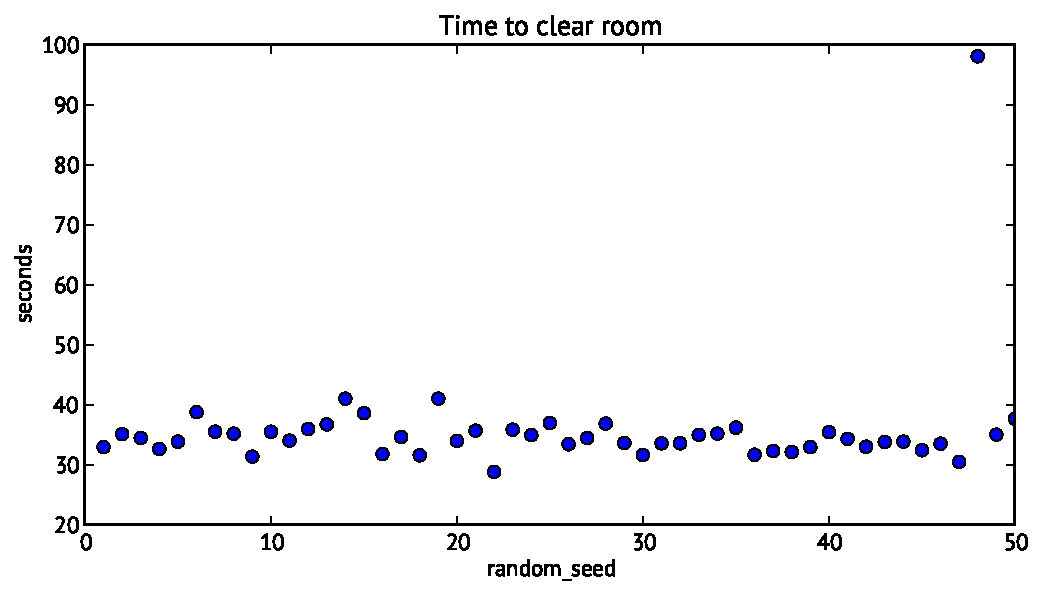
\includegraphics[width=0.8\textwidth]{Figures/random-seed-variations.pdf}
    \caption[Leaving time for different random seeds]{Leaving time for 
    different random seeds. Results are dependent on random numbers; for a 
    seed value of 48 (top-right corner), one pedestrian starts out walking 
    very slowly impacting the total leaving time.}
    \label{fig:random-seed}
\end{figure}


\subsection{Summary}
We have discussed several possible cause for errors in our model, and possible 
remedies. The forces in the model have a simplistic nature in that they only 
have one direction, corresponding to the direction between the repulsion 
points, and they are not adjusted by pedestrian walking speed. This could be 
remedied by adding tangential forces and forces that are dependent on walking 
speed, which might produce better results. Selection of parameters is also a 
possible source of error; a possible remedy, that is inaccessible to us, is 
obtaining parameters from real-world experiments, by fitting data to 
simulations. Finally, errors arising from the nature of our implementation 
might occur. This includes possible coding errors, and errors as a result of 
extremely small or large random numbers used when setting initial conditions. 
This can be somewhat mitigated by testing the implementation, and by 
discarding very small or large random numbers.

In the next section we asses social force models based on our results and the 
error sources discussed in this section.
